%%%%%%%%%%%%%%%%%%%%%%%%%%%%%%%%%%%%%%%%%%%%%%%%%%%%%%%%%%%%%%%%%%%%%%%%%%%%%%%%
%% SUBSECTION: Metodologia badania
%%%%%%%%%%%%%%%%%%%%%%%%%%%%%%%%%%%%%%%%%%%%%%%%%%%%%%%%%%%%%%%%%%%%%%%%%%%%%%%%
\subsection{Metodologia badania}

Podstawą badania zużycia energii jest pomiar wartości pobieranego prądu przez zestaw uruchomieniowy
P-NUCLEO-WB55 w czasie. Posiadając dane wymienione dane, na podstawie oczywistych
zależności fizycznych, wyznacza się parametry jak całkowita wykorzystana energia
podczas badania, przedstawiona w przystępnej formie parametru mocy.

Pomiary wartości chwilowego poboru prądu oparto o moduł opisany w punkcie~\ref{device:plytka_pomiarowa}.
Źródłem energii dla płytki pomiarowej jest komputer klasy PC, a precyzyjniej udostępniany
port USB. Wykorzystując również ten protokół następuje transmisja danych poprzez komunikację szeregową
UART, umożliwiając akwizycję danych.

Połączenie z zestawem uruchomieniowym oparto o konektor CN14 udostępniający piny: PIN1 - masa GND, PIN3 - VCC $3.3V$~\cite{noauthor_um2243_2018}.
Wyprowadzone przewody połączono następnie z P-NUCLEO-WB55 poprzez konektor JP2, wcześniej pozbawiony zawleczki.
Jest to metoda rekomendowana dla pomiaru prądu opisana w dokumentacji zestawu~\cite{stmicroelectronics_um2435_2019}\footnote{
Rozdział 7.12 Current measurement}. Porty kompatybilne z Arduino/ST Morpho mogłyby stanowić równorzędny sposób
włączenia zestawu uruchomieniowego do obwodu płytki pomiarowej. Autorska analiza dokumentacji sugeruje jednak,
iż opcja ta nie jest wspierana. Wymagane byłoby lutowanie dodatkowego połączenia w (punkcie SB27), by móc wykorzystać
zasilanie napięciem $3.3V$.

\begin{figure}[!ht]
	\centering 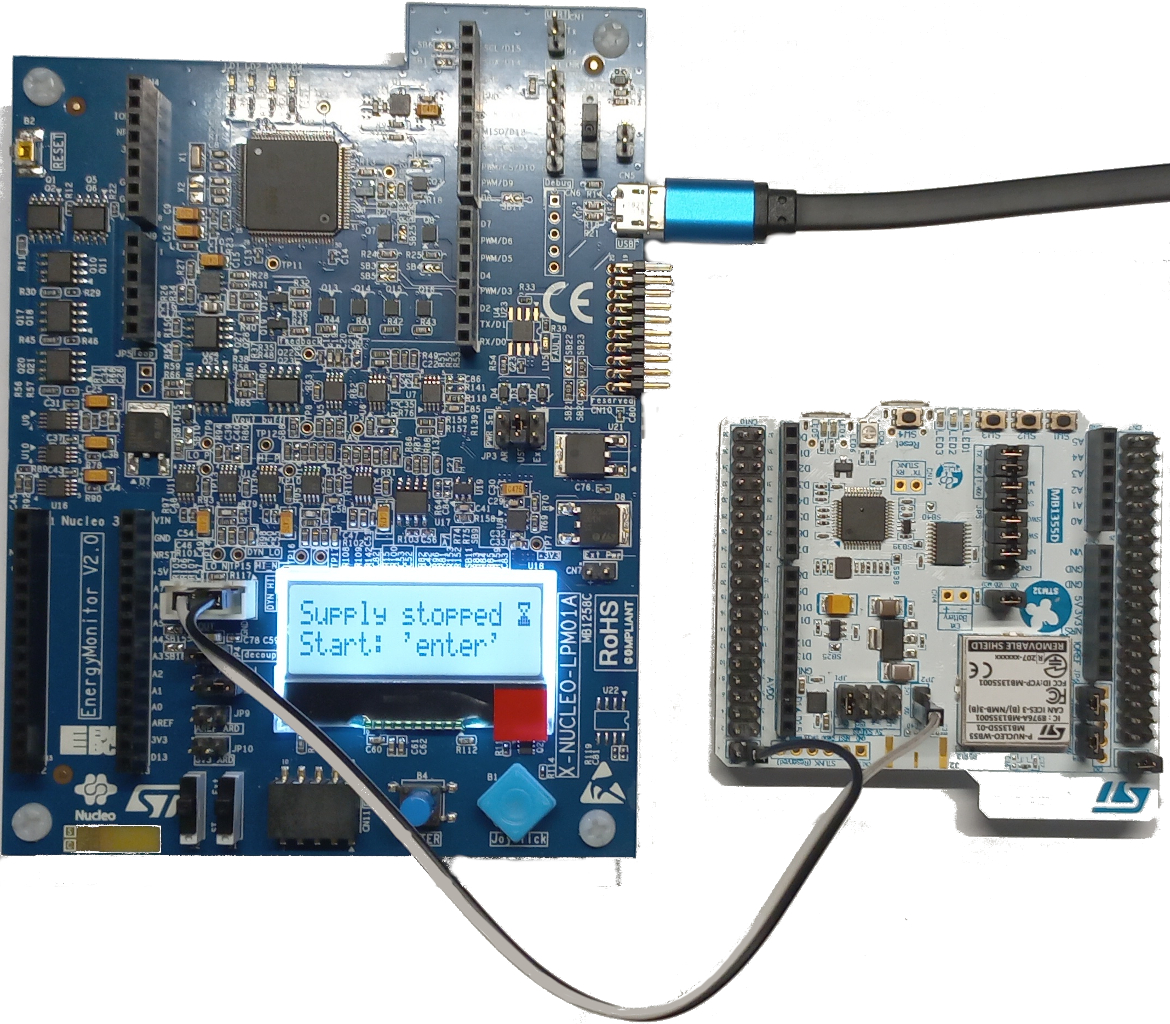
\includegraphics[width=0.618\linewidth]{power_measurement_unit_connected.png}
	\caption{Podłączony zestaw pomiarowy}
	\label{rys:connected_power_measurement_unit}
\end{figure}

Celem akwizycji danych, wybrano dostarczane przez producenta oprogramowanie \textit{STM32CubeMonitor-Power}.
Przykładowy zrzut ekranu zaprezentowany jest na rysunku~\ref{rys:measurement_session_sample}.
Pojedyncza sesja pomiarowa trwająca 100 sekund zapewnia niezbędne dane. Są one następnie
odpowiednio przetwarzane poprzez odcięcie wartości zebranych w ostatnich sekundach. Związane to było
ze sposobem działania mikrokontrolera, który po 60 sekundach domyślnie przechodzi w stan zwiększonej
oszczędności energii (Low Power Advertising). Parametr ten można zmienić wg własnych upodobań, aczkolwiek zdecydowano
się na domyślne nastawy, tak by umożliwić możliwie proste, ponowne przeprowadzenie doświadczenia wykorzystując przykład
BLE \gls{HRT} dostarczony przez ST. Stąd, by rozróżnić różne tryby pracy \gls{BLE}, zdecydowano o odcięciu
połowy okresu pomiarowego, zapewniając jednolite wartości względem trybów zużycia energii
w~50 sekundowym oknie.

Tak zebrane dane następnie przetworzono uzyskując wartości energii i średniej mocy
użytej przez układ. Wykorzystuje się w celu oczywistą zależność fizyczną zaprezentowaną
wzorem~\ref{energy_equation}~\cite{skoro_marta_fizyka_1973}.

\begin{equation} \label{energy_equation}
E_{\text{całkowita}} = U \cdot \int_{t=0[s]}^{t=50[s]} \mathrm{d}i \: \mathrm{d} t
\end{equation}

\begin{equation} \label{power_equation}
P = \frac{E_{\text{całkowita}}}{t}
\end{equation}

gdzie:

\begin{description}
\item $E_{\text{całkowita}} [J]$ - wykorzystana energia podczas 50s sekundowej sesji rejestracji danych
\item $P [W]$ - moczużyta podczas 50s sekundowej sesji rejestracji danych
\item $U [V]$ - napięcie zasilania mikrokontrolera - 3.3V - stała
\item $\mathrm{d}i [A]$ - prąd w danej chwili
\item $\mathrm{d}t [s]$ - podstawa czasowa całkowania, 0.01s/interwał (100Hz) - stała 
\end{description}

Zebrane dane w postaci wartości chwilowych pobieranego przez mikrokontroler prądu względem czasu
przetworzono z użyciem metod numerycznych. W~celu wyliczenia łącznej wykorzystanej energii, a~tym samym
mocy, stosuje się zależność~\ref{energy_equation}. Uwzględniając fakt działania w domenie dyskretnej,
wykorzystano kompozytową metodę całkowania Simpsona~\cite{noauthor_scipyintegratesimpson_nodate}.
Podstawą dla całkowania są wartości zebrane w równoodległych odstępach. Dokonując akwizycji danych,
dobrano częstotliwość próbkowania jako $100Hz$. Każda kolejna wartość charakteryzuje się więc
10 milisekundową różnicą w~podstawie czasu. Uwzględniając ten fakt, wyliczenie wartości
wykorzystanej energii jak i~mocy staje się trywialne.

\begin{figure}[!ht]
	\centering 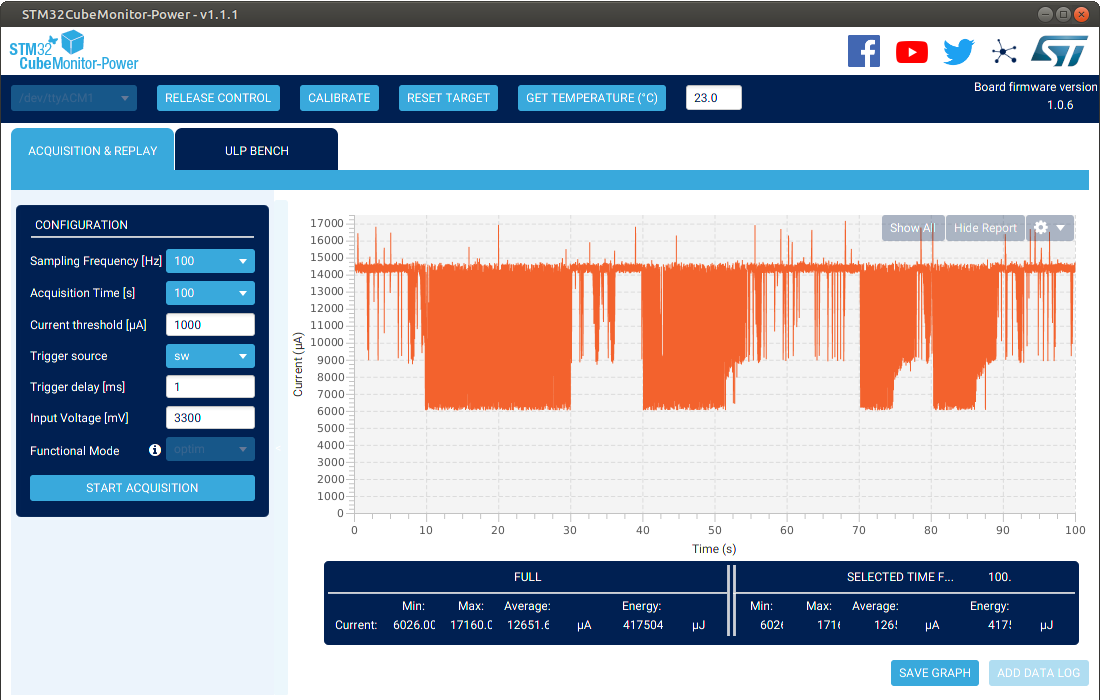
\includegraphics[width=0.618\linewidth]{stm32_power_monitor_sample.png}
	\caption{Przykładowa sesja pomiarowa dla BLE Mesh - sieć w trybie nasłuchującym}
	\label{rys:measurement_session_sample}
\end{figure}


%%%%%%%%%%%%%%%%%%%%%%%%%%%%%%%%%%%%%%%%%%%%%%%%%%%%%%%%%%%%%%%%%%%%%%%%%%%%%%%%
%% SUBSECTION: BT Low Energy - Usługa Heart Rate
%%%%%%%%%%%%%%%%%%%%%%%%%%%%%%%%%%%%%%%%%%%%%%%%%%%%%%%%%%%%%%%%%%%%%%%%%%%%%%%%
\subsection{BT Low Energy - Usługa Heart Rate}

Pierwszą usługą BLE badaną pod kątem zużycia energii jest Heart Rate\footnote{z ang. rytm serca}. Wybór
ten podyktowany jest chęcią przyszłego zestawienia wartości z~rozwiązaniami innych producentów.
Usługa zdefiniowana przez Bluetooth SIG stanowi więc wspólny międzyplatformowy język.
Porównanie konkurencyjnych rozwiązań względem ST stanowi potencjalny kierunek dalszych rozważań.

Badania przeprowadzono dla trzech różnych trybów działania aplikacji BLE HRT:
\begin{itemize}
\item Usługa połączona (Connected)
\item Usługa w trybie szybkiego ogłaszania (Fast Advertising)
\item Usługa w trybie niskomocowego ogłaszania (Low Power Advertising)
\end{itemize}

Emitowana moc ustalona została na $-0.15dBm$. Jest to wartość wspólna dla każdego pomiaru
dotyczącego BLE HRT.

Rysunek~\ref{rys:power_ble_hr_connected_only_amps} przedstawia charakterystykę poboru prądu
w czasie po ustanowieniu połączenia urządzeniem klienckim. Mikrokontroler publikuje 
losowe dane z częstotliwością $1Hz$. W konsekwencji radio zestawu uruchomieniowego
uruchamiane jest co najmniej raz na sekundę.

Analizując wykres dostrzega się regularne, 10-sekundowe interwały w których pobierany prąd dąży do swojego
maksimum wynoszącego ok. $12mA$. Jest to prawdopodobnie związane z ustawionymi parametrami transmisji
danych w mikrokontrolerze. Niniejsza praca nie podejmuje jednak próby wyjaśnienia rzeczywistej przyczyny tego zjawiska.
Minimalny zarejestrowany pobór prądu ustalony jest na ok. $422uA$, czyli o dwa rzędy wielkości mniejsze wartości
szczytowej.


\begin{figure}[!ht]
	\centering 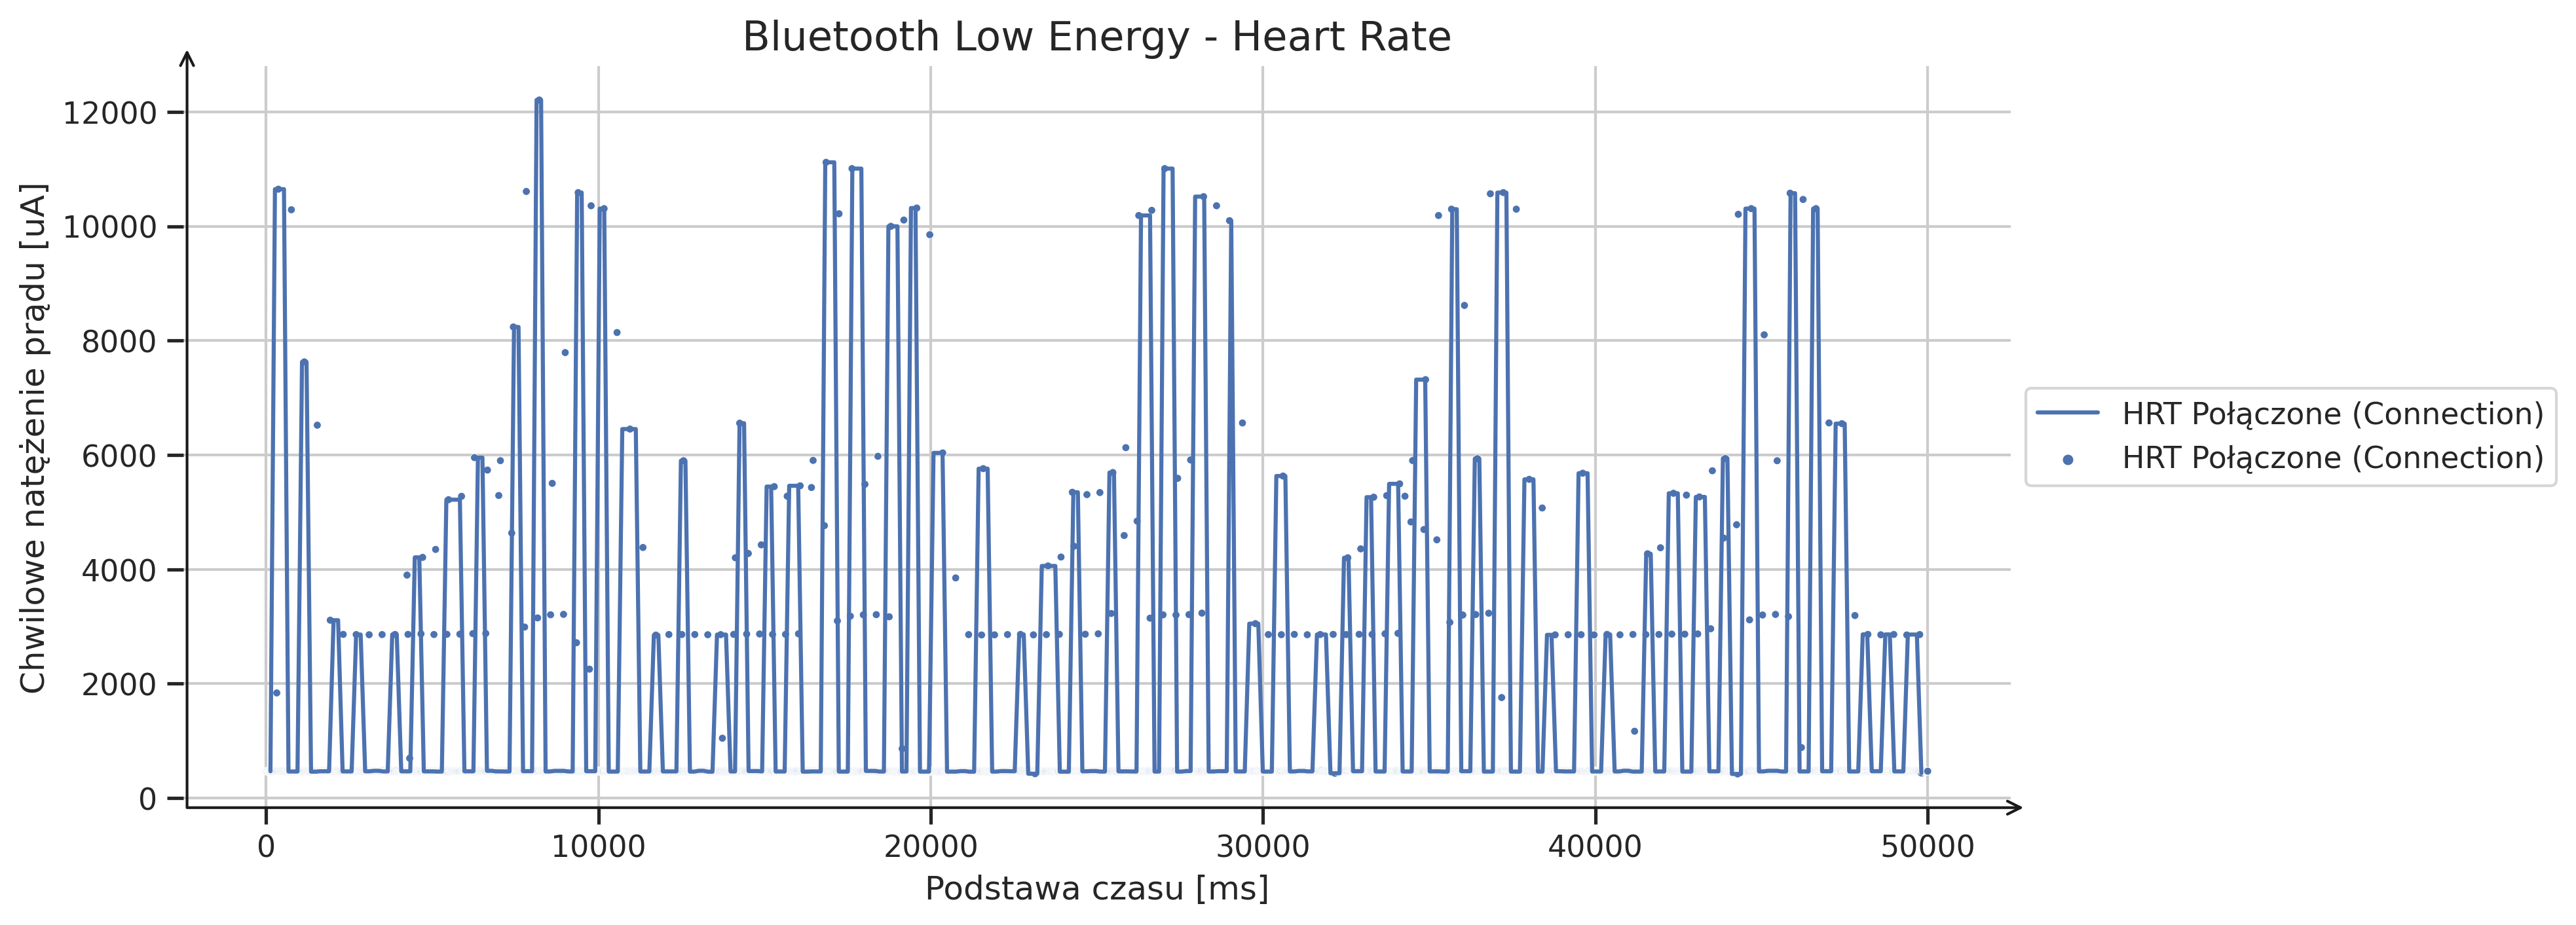
\includegraphics[width=0.99\linewidth]{power_ble_hr_connected_only_amps.png}
	\caption{Charakterystyka czasowa poboru prądu dla BLE i usługi Heart Rate - Usługa Połączona}
	\label{rys:power_ble_hr_connected_only_amps}
\end{figure}

Rysunek~\ref{rys:power_ble_hr_fastadv_only_amps} przedstawia charakterystykę poboru prądu po czasie
dla szybkiego trybu ogłoszeniowego. Zgodnie za kodem źródłowym, interwały w których rozgłaszane
są komunikaty powinny się zawierać w częstości od 80 do 100ms. Wywołuje to konieczność uruchamiania radia
co najmniej 10 razy na sekundę. Ma to swoje odzwierciedlenie na wykresie. Charakterystyka jest bardziej
\textit{burzliwa} w porównaniu z wykresem~\ref{rys:power_ble_hr_connected_only_amps}. 

Zauważa się większą częstotliwość szczytów osiągających wartości pomiędzy $10-12mA$. Jest to w~oczywisty
sposób powiązanie ze sposobem działania trybu \textit{Fast Advertising}. Minimalna wartość zarejestrowana wynosi jednak
$350uA$, co ponownie stanowi różnicę dwóch rzędów wielkości.

\begin{figure}[!ht]
	\centering 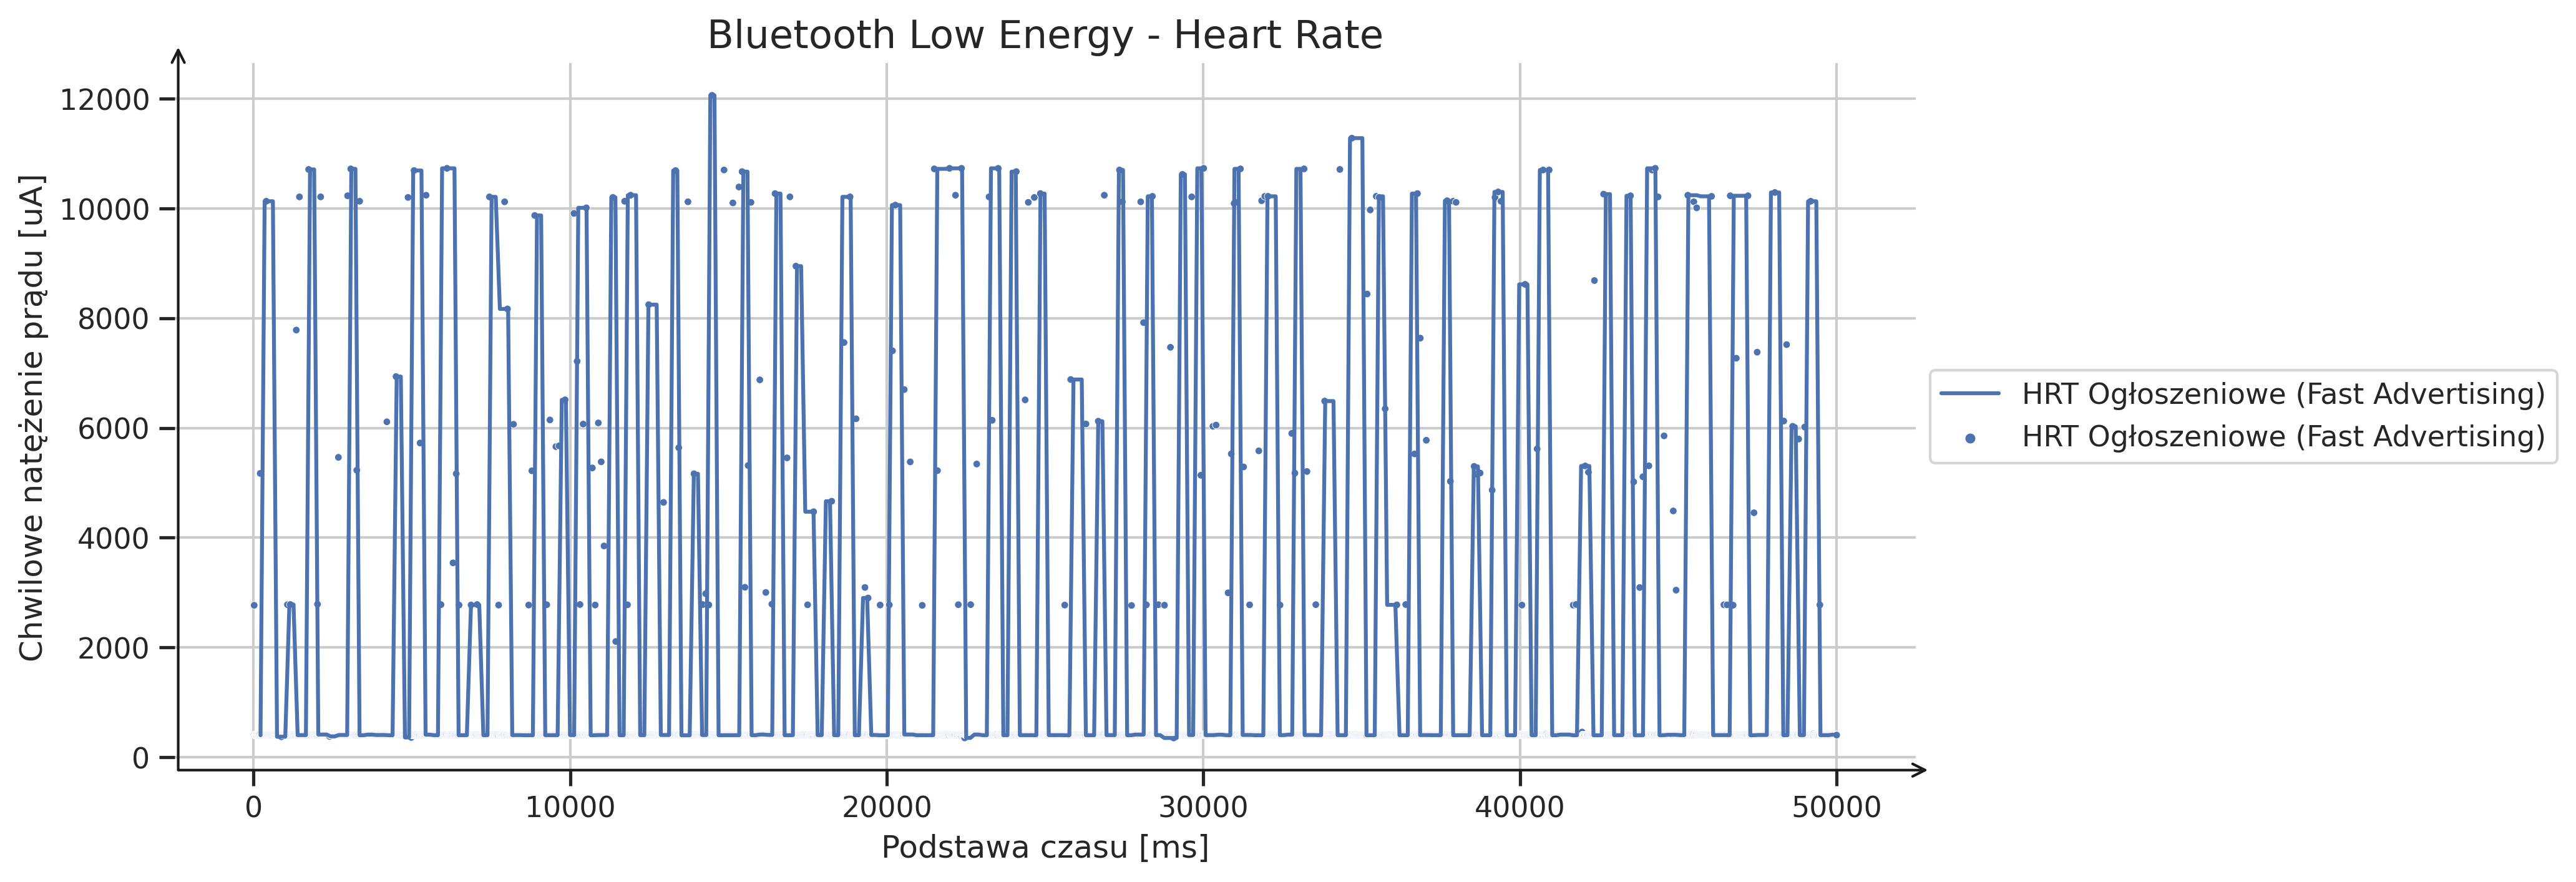
\includegraphics[width=0.99\linewidth]{power_ble_hr_fastadv_only_amps.png}
	\caption{Charakterystyka czasowa poboru prądu dla BLE i usługi Heart Rate - Tryb szybkiego ogłaszania}
	\label{rys:power_ble_hr_fastadv_only_amps}
\end{figure}

Ostatnim wykresem prezentującym charakterystykę poboru prądu w czasie jest rysunek~\ref{rys:power_ble_hr_low_power_adv_only_amps}.
Przedstawia on tryb działania niskomocowego ogłaszania. Różni się on względem trybu \textit{Fast Advertising} częstością z jaką wysyłane
są pakiety ogłoszeniowe. W tym przypadku, oprogramowanie wysyła wiadomości z interwałem znajdującym się w przedziale od 
jednej do dwóch i~pół sekundy (parametry: \textit{\texttt{CFG\_LP\_CONN\_ADV\_INTERVAL\_MIN}} i \textit{\texttt{CFG\_LP\_CONN\_ADV\_INTERVAL\_MAX}}). 
Oba wymienione tryby są autorskim rozwiązaniem ST. Przegląd literatury nie wskazuje, jakoby takie zachowanie wymagane
jest przez sam standard.

Rysunek~\ref{rys:power_ble_hr_low_power_adv_only_amps} wskazuje na podobne zależności. Obserwuje się periodyczne, aczkolwiek
stosunkowo rzadkie szczyty w poborze energii rozumianej jako przepływ prądu elektrycznego. Wpisują się jednak w~wyżej wymienione
parametry transmisji. Brak całkowitego dopasowania względem oczekiwanych parametrów może być spowodowany niedostateczną
częstotliwością próbkowania. Z pewnością jest to zagadnienie, które warto przeanalizować w kolejnych iteracjach prób doświadczalnych.


\begin{figure}[!ht]
	\centering 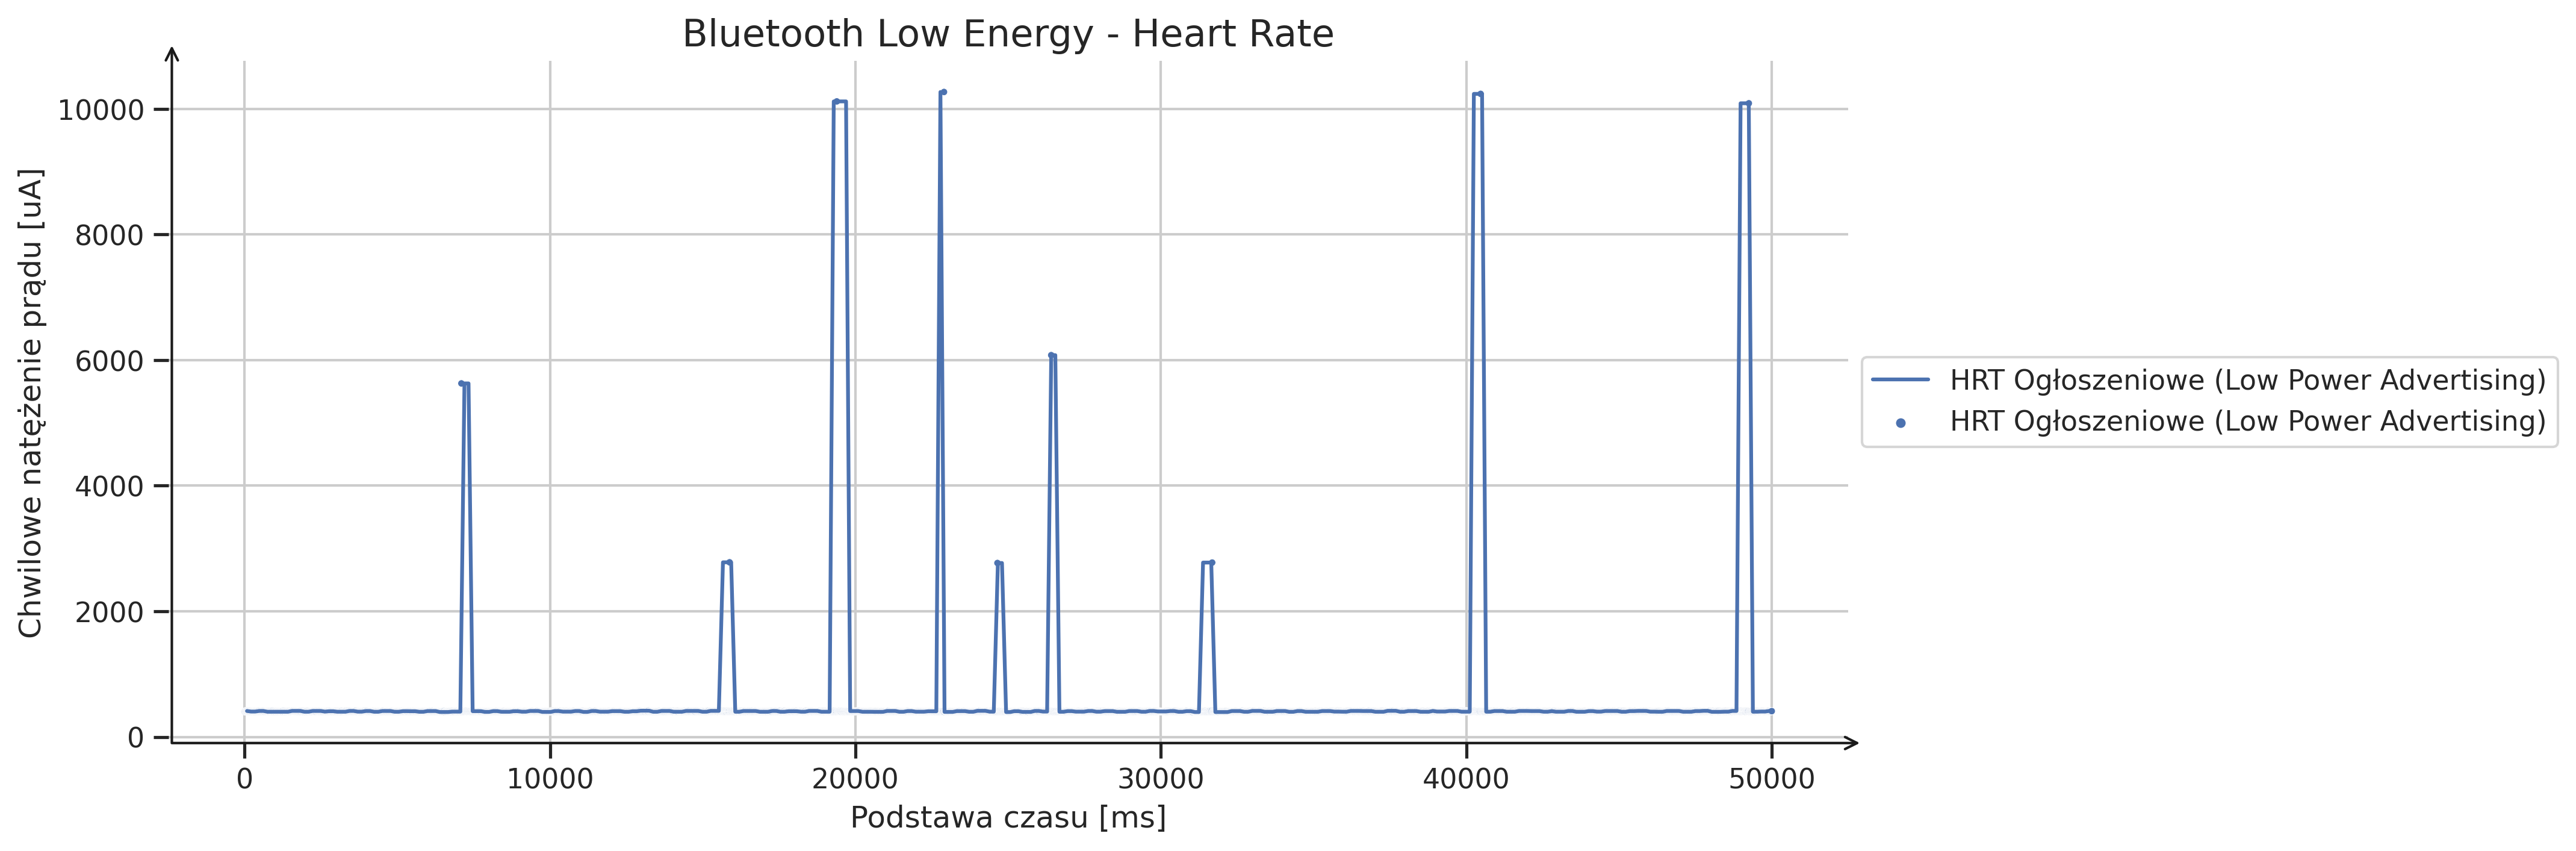
\includegraphics[width=0.99\linewidth]{power_ble_hr_low_power_adv_only_amps.png}
	\caption{Charakterystyka czasowa poboru prądu dla BLE i usługi Heart Rate - Tryb niskomocowego ogłaszania}
	\label{rys:power_ble_hr_low_power_adv_only_amps}
\end{figure}

Ostatecznie, zestawia się wszystkie zebrane jak dotąd wartości pomiarowe na rysunku~\ref{rys:power_ble_hr_amps_usage_juxtaposition}.
Wykres słupkowy przedstawia średni pobór prądu wyrażony miliamperach. Porównując, zauważa się znaczącą, blisko dwukrotną
różnicę, co do zużytej mocy, pomiędzy trybem ogłoszeniowym niskomocowym a~pozostałymi kategoriami.

Porównując wymienione tryby ogłoszeniowe, należy zwrócić uwagę na konfigurację częstotliwości, z którą wysyłane są
pakiety danych. Częstotliwość, z którą aktywowane jest radio, może być nawet 30 krotnie wyższa dla przypadku szybkiego ogłaszania.
Uwidocznia się również różnica w maksymalnie osiągniętym szczycie poboru mocy, wynosząca ok. $2mA$.

\begin{figure}[!ht]
	\centering 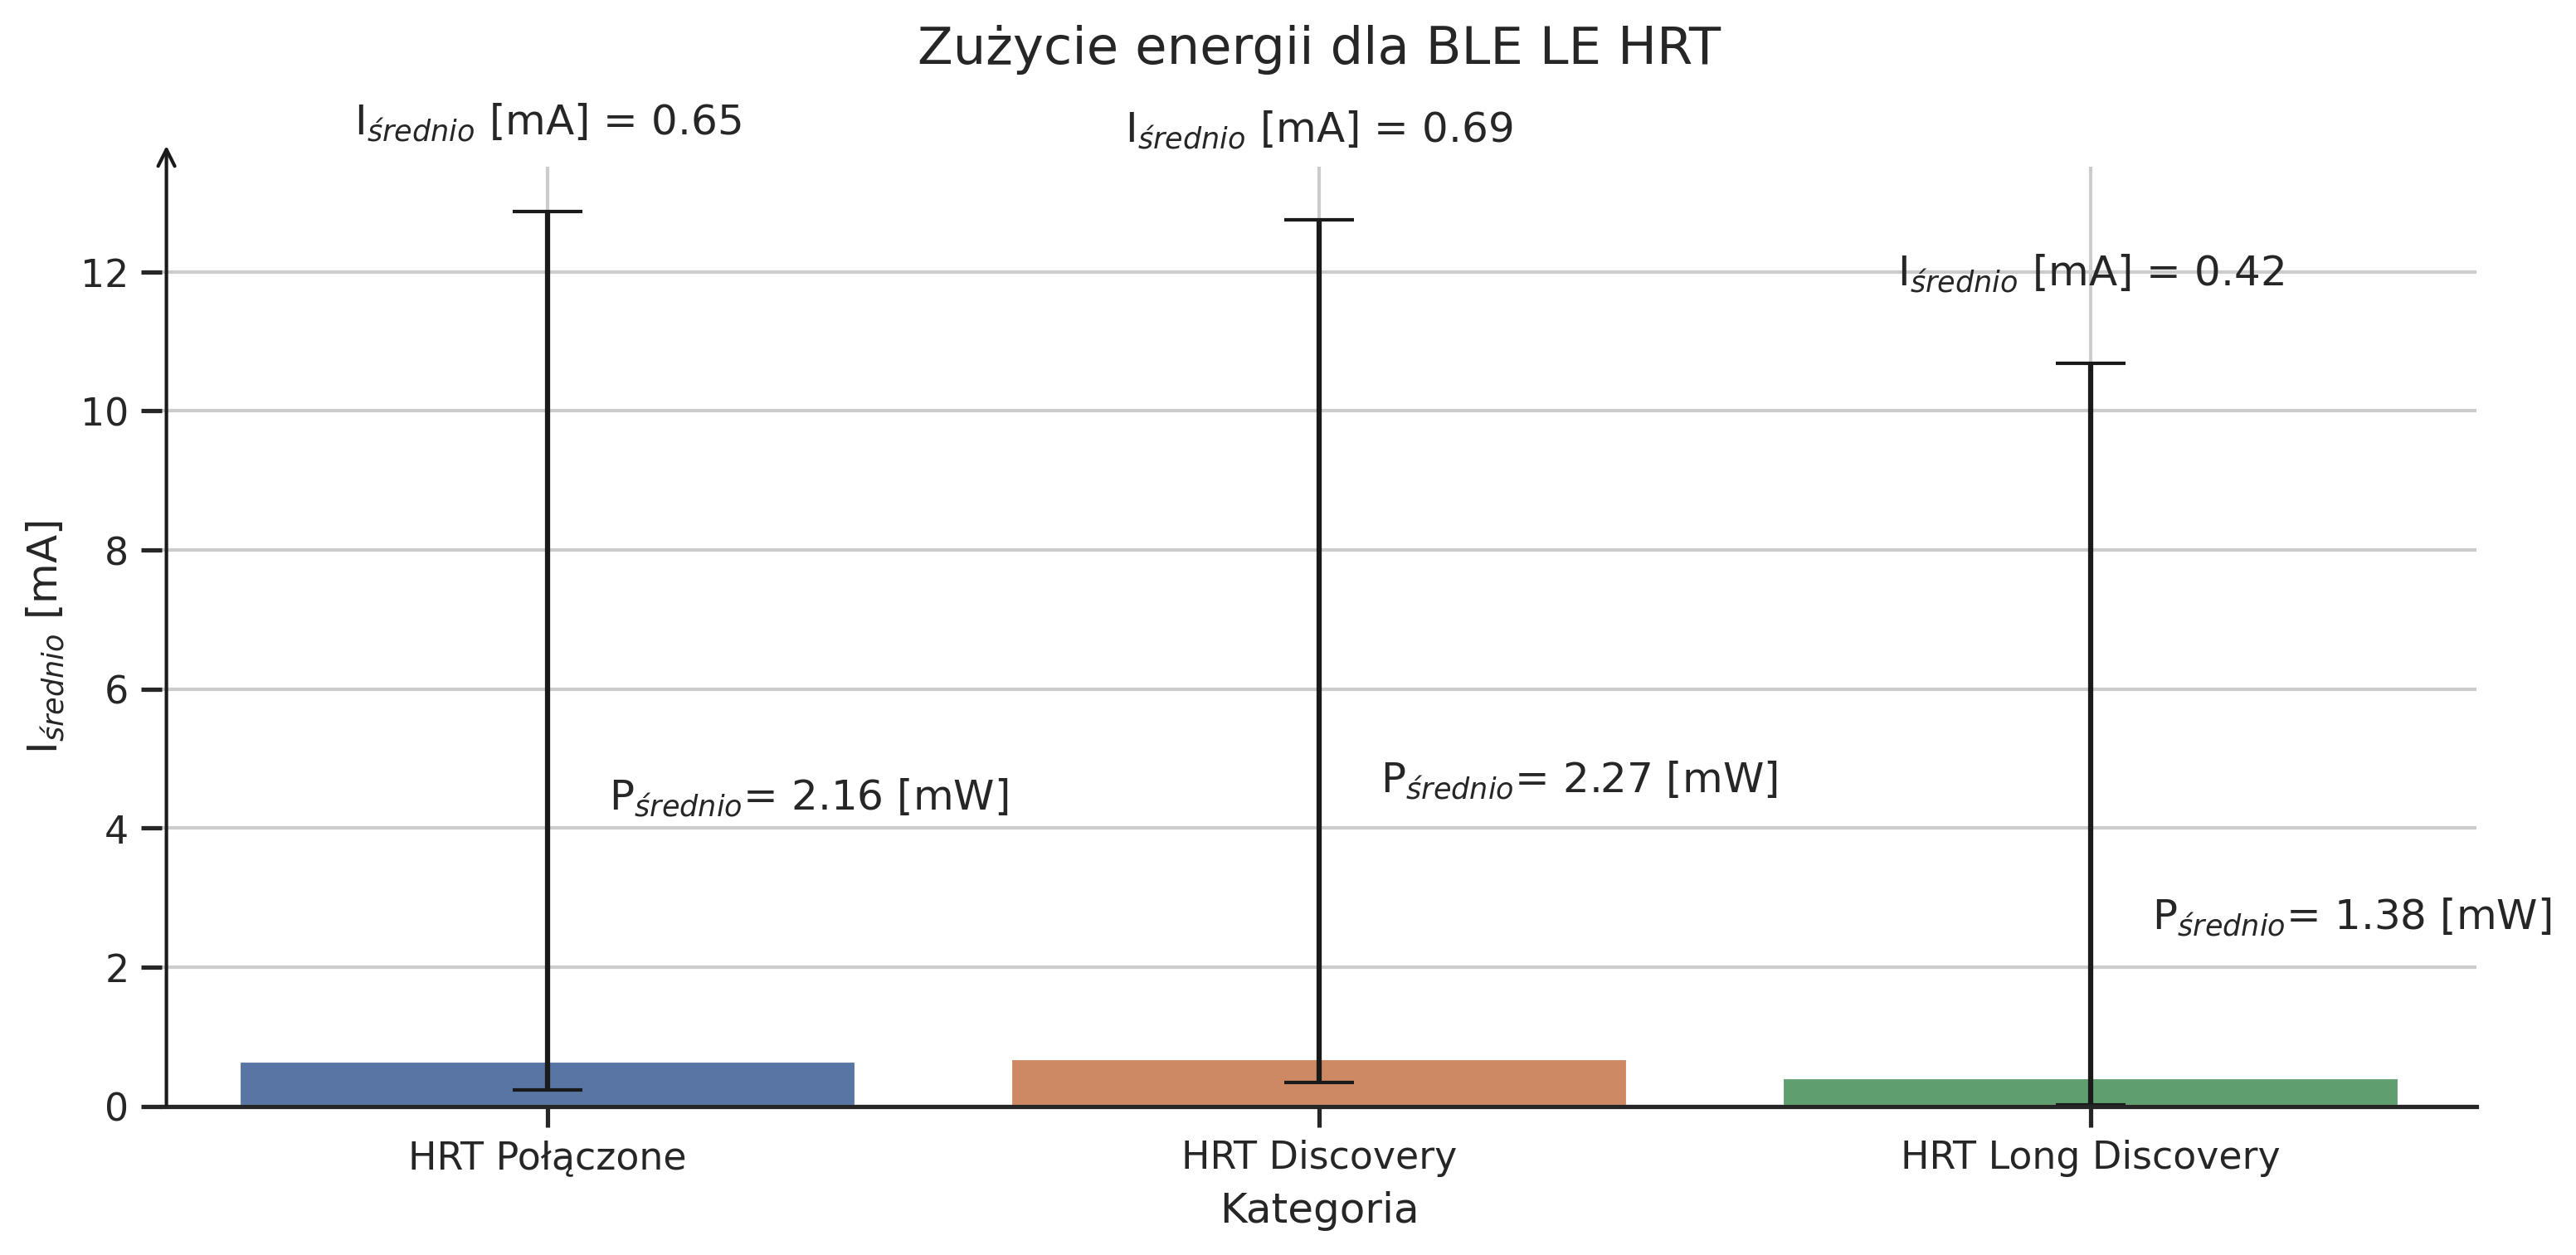
\includegraphics[width=0.99\linewidth]{power_ble_hr_amps_usage_juxtaposition.png}
	\caption{Zestawienie zużycia prądu dla usługi Heart Rate w zależności od trybu działania}
	\label{rys:power_ble_hr_amps_usage_juxtaposition}
\end{figure}

Zużycie energii w zestawieniu trybu ogłoszeniowego szybkiego i ustanowionego już połączenia jest zbliżone. Według zadanych nastawień,
\textit{Fast Advertising} aktywuje radio około 10 razy częściej aniżeli po ustanowieniu łączności z aplikacją kliencką. Natomiast,
przypadek połączonej już usługi przenosi dodatkowe informacje takie jak puls czy estymowana spalona energia w wyników procesów
metabolicznych. Być może, zużycie energii również zależy od ilości przenoszonych danych, a~co za tym idzie, 
wydłużenia czasu działania radia niezbędnego do wysłania takiej wiadomości. Jest to pytanie otwarte.

%%%%%%%%%%%%%%%%%%%%%%%%%%%%%%%%%%%%%%%%%%%%%%%%%%%%%%%%%%%%%%%%%%%%%%%%%%%%%%%%
%% SUBSECTION: BLE Mesh - Model Generic OnOff
%%%%%%%%%%%%%%%%%%%%%%%%%%%%%%%%%%%%%%%%%%%%%%%%%%%%%%%%%%%%%%%%%%%%%%%%%%%%%%%%
\subsection{BLE Mesh - Model Generic OnOff}

Zużycie energii dla \gls{BLE} Mesh przeprowadzono dla dwóch wariantów:
\begin{itemize}
\item sieć w trybie gotowości (\textit{standby})
\item sieć w której wysyłany jest komunikat z modelu \textit{Generic OnOff}
\end{itemize}

Poprzez sieć w trybie gotowości należy rozumieć, iż wszystkie zarejestrowane\footnote{proces w anglojęzycznej literaturze i dokumentacji znany jest jako \textit{provisioning}}
węzły są uruchomione. Zgodnie ze standardem BLE Mesh, każdy z~takich węzłów musi mieć zaimplementowane dwa modele:
\textit{Configuration Server} i~\textit{Health Server} \cite{wooley_martin_bluetooth_2019}. 
Odpowiadają one za niezbędną konfigurację jak i~również nadzorowanie stanu \textit{zdrowia} sieci, poprzez wysyłanie 
komunikatów \textit{keep-alive}\footnote{standard definiuje takie komunikaty jako \textit{heartbeats}\cite{wooley_martin_bluetooth_2019}\cite{mesh_working_group_mesh_2019}}.

Rozpatrywany przypadek \textit{Generic OnOff} wykorzystuje tenże model do wysyłania komunikatów wewnątrz sieci.
Jeden z węzłów wysyła pakiet danych a~drugi, odbiorczy, przetwarza wykonując operację zdefiniowaną przez model akcję.
W~przypadku poniższych badań operacją tą jest kolejne zliczanie otrzymanych pakietów.
W~tym celu wykorzystano oprogramowanie opracowane na potrzeby kolejnego opisywanego eksperymentu \textit{Packet Error Rate}.
Przez cały okres akwizycji wysyłano komunikaty z~częstotliwością $2Hz$. Zasadne jest wspomnieć, iż na czas trwania doświadczenia wszelkie 
diody emitujące światło zostały wyłączone celem eliminacji błędów systemowych wpływających na ostateczne zużycie energii przez
urządzenie.

\begin{figure}[!ht]
	\centering 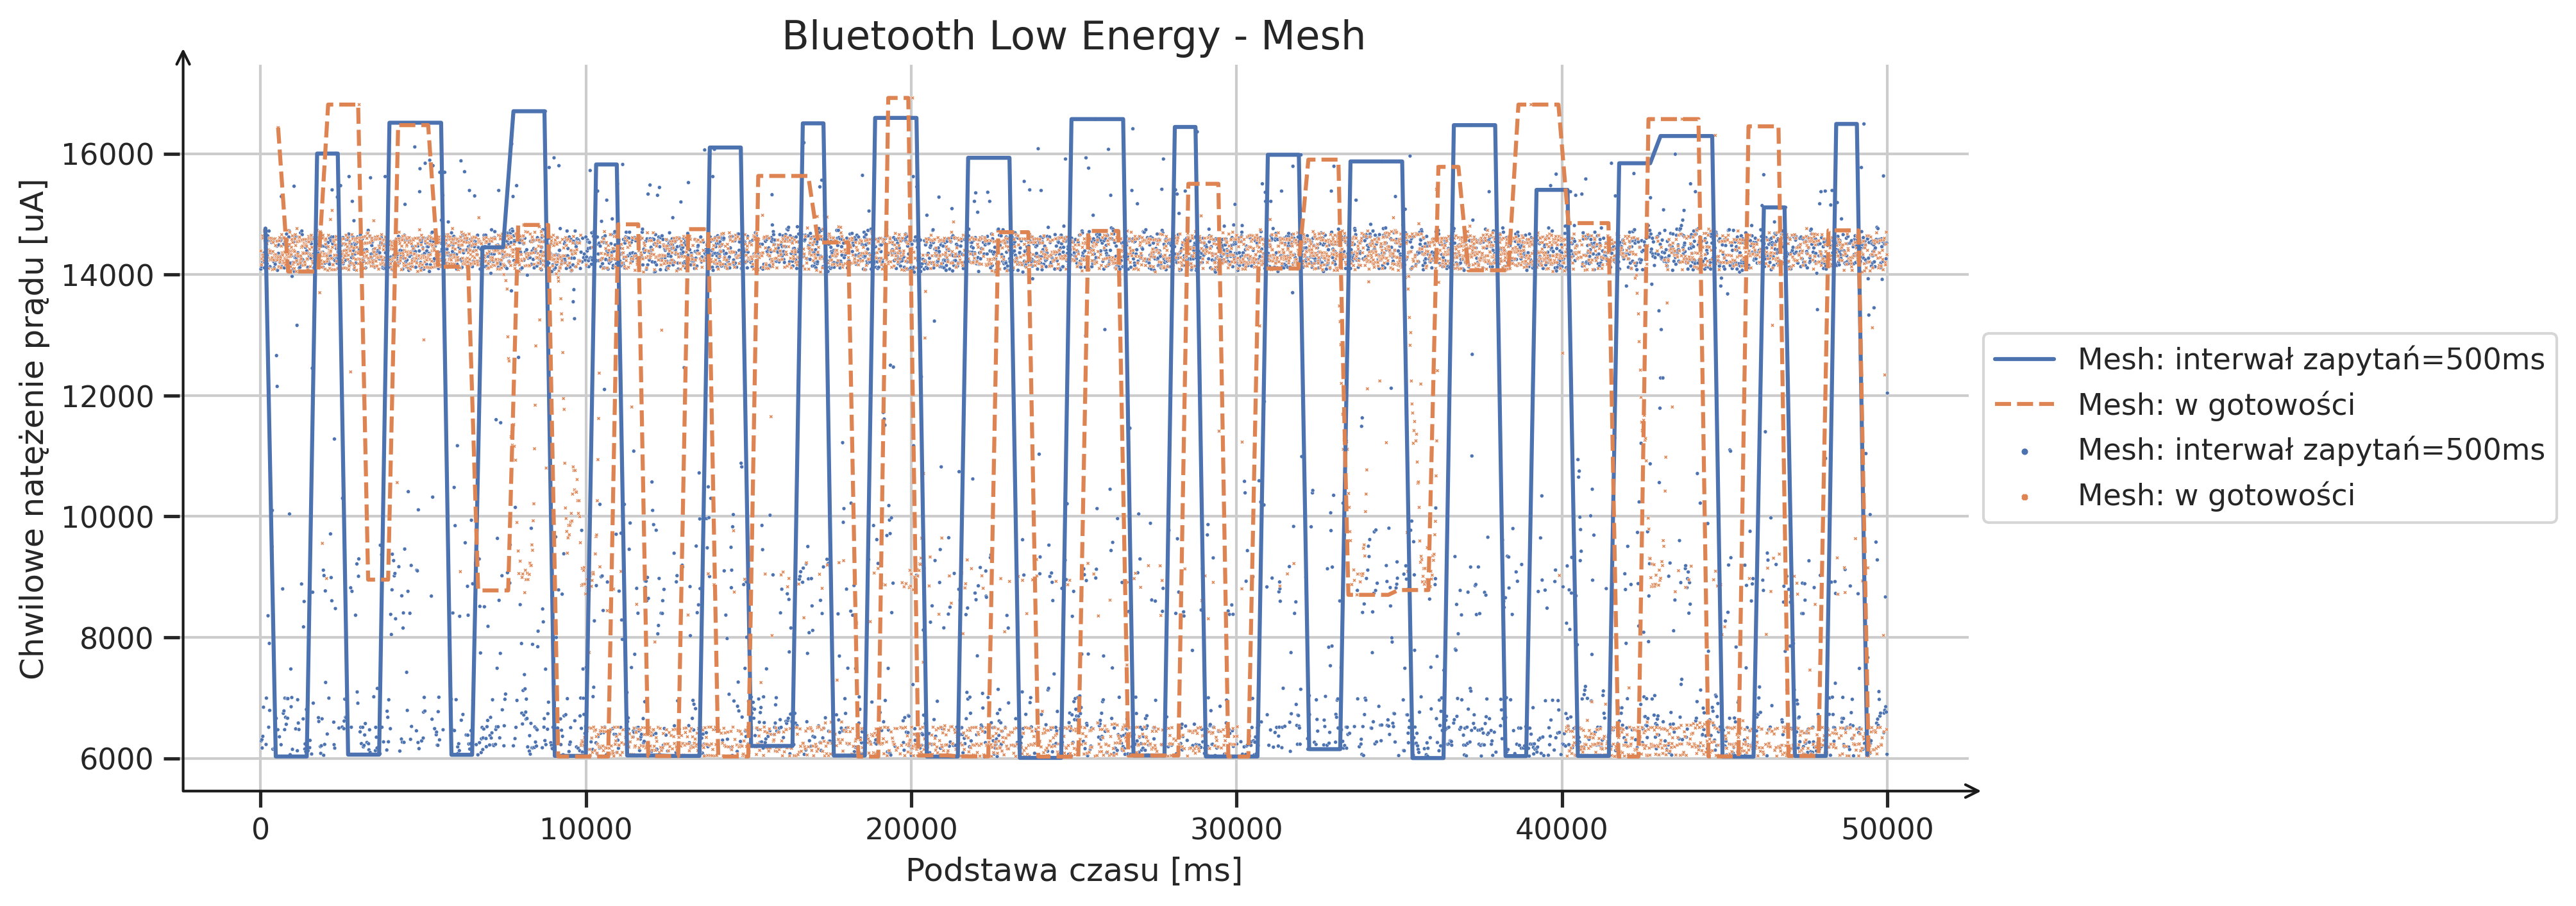
\includegraphics[width=0.99\linewidth]{power_ble_mesh_amps_no_led.png} 
	\caption{Charakterystyka czasowa poboru prądu dla BLE Mesh i modelu Generic OnOff}
	\label{rys:power_ble_mesh_amps}
\end{figure}


Rysunek~\ref{rys:power_ble_mesh_amps} przedstawia charakterystyki prądu dla wymienionych wcześniej badanych wariantów. Wartości są aproksymowane
celem wskazania ogólnej zmiennej tendencji poboru prądu elektrycznego. Jej zmienność reprezentuje wykres punktowy, zlewający się 
w~trzy rozpoznawalne klastry oscylujące wokół wartości $14mA$, $9mA$ i $6mA$. Rzeczywista charakterystyka wygenerowana przez
aplikację \textit{STM32CubeMonitor-Power} zaprezentowana jest na rysunku~\ref{rys:power_ble_mesh_standby_powermonitor}.

\begin{figure}[!ht]
	\centering 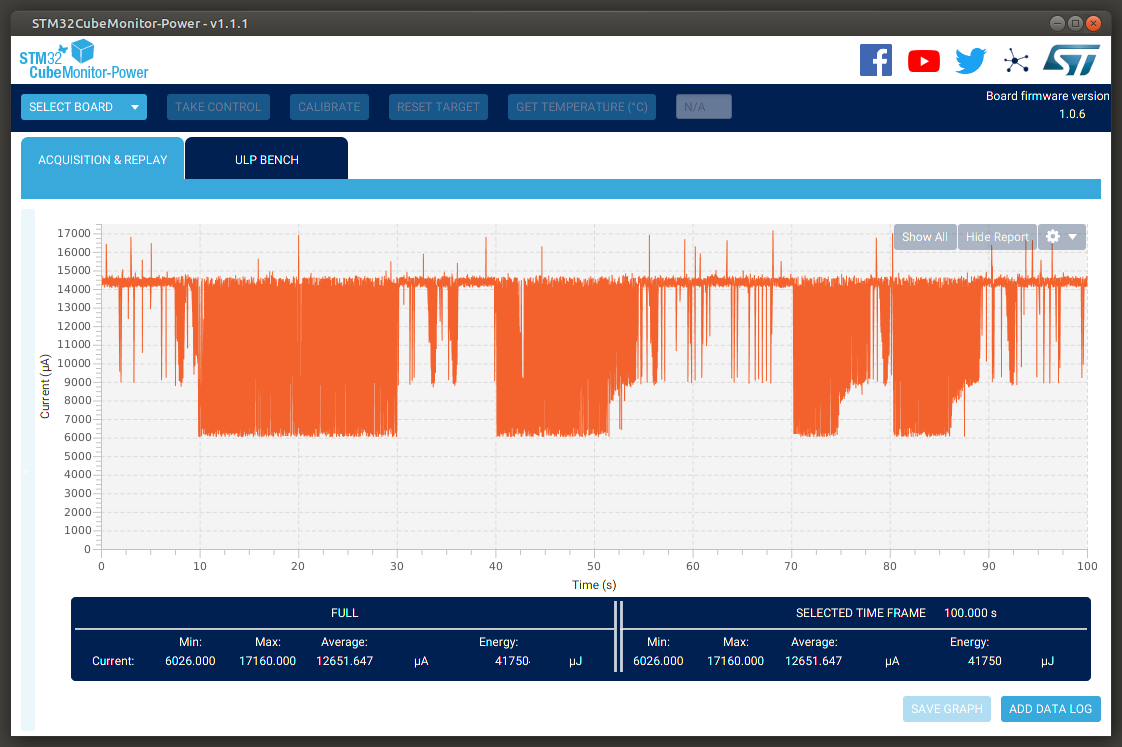
\includegraphics[width=0.618\linewidth]{power_ble_mesh_standby_powermonitor.png} 
	\caption{Rzeczywista charakterystyka poboru energii dla BLE Mesh działającego w trybie gotowości}
	\label{rys:power_ble_mesh_standby_powermonitor}
\end{figure}

Rysunek~\ref{rys:power_ble_mesh_standby_powermonitor} wygenerowany przez aplikację produkcji \textit{ST} odpowiada chmurze punktów
z~rysunku~\ref{rys:power_ble_mesh_amps} dla wariantu regularnych zapytań co 500ms. Analogiczny wykres dla
trybu nasłuchującego wygenerowany przez \textit{STM32CubeMonitor-Power} reprezentowany jest na rysunku~\ref{rys:measurement_session_sample}.
Swoiste zagęszczenie punktów pomiarowych i~częste zmiany amplitudy mogą wskazywać na złożoność protokołu Mesh,
który wymaga częstych operacji w tym radiowych. Operacje te bezpośrednio oddziałują na zużycie energii, co w~oczywisty
sposób widoczne jest na wykresach.


\begin{figure}[!ht]
	\centering 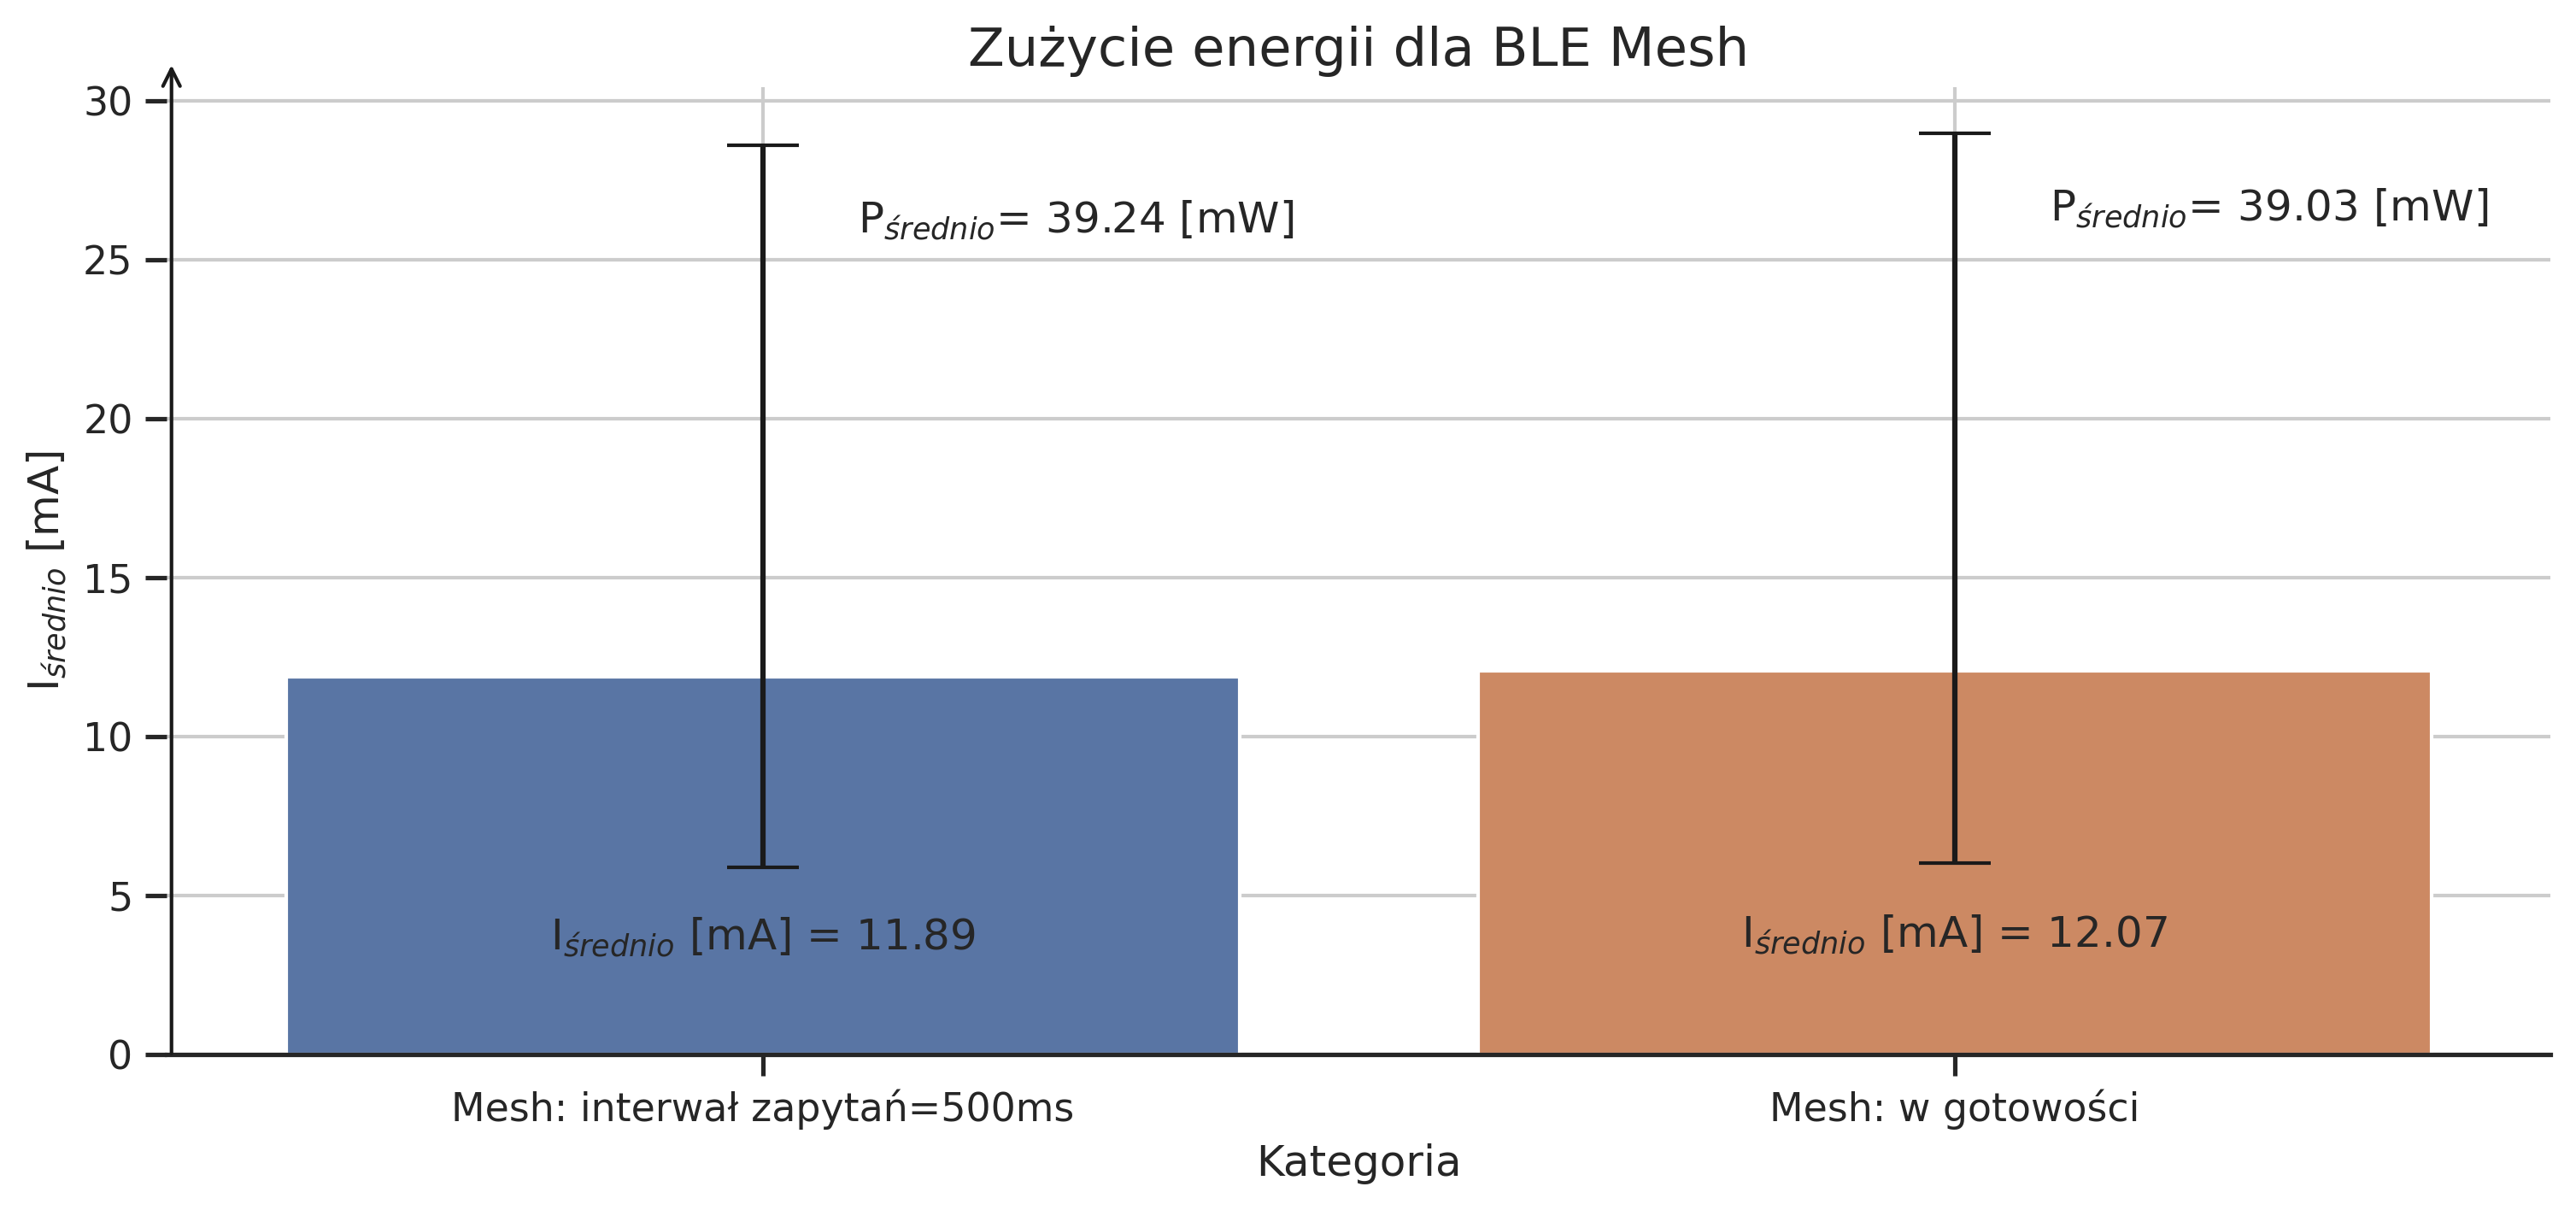
\includegraphics[width=0.99\linewidth]{power_ble_mesh_amps_usage_juxtaposition_no_led.png} 
	\caption{Zestawienie zużycia prądu dla BLE Mesh w zależności od trybu działania}
	\label{rys:power_ble_mesh_amps_usage_juxtaposition}
\end{figure}

Parametry zużycia energii przedstawia rysunek~\ref{rys:power_ble_mesh_amps_usage_juxtaposition}. Porównywane są dwa zdefiniowane
warianty działania aplikacji. Uwidacznia się niewielka różnica konsumowanej mocy. Węzeł odbierający komunikaty \textit{Generic OnOff}
wymaga średnio 39,2mW mocy do funkcjonowania. Konkurencyjny wariant potrzebuje jej nieznacznie mniej. Mesh będący w gotowości
potrzebuje średnio 39.0mW mocy. Minimalne i maksymalne natężenia chwilowo pobieranego prądu są porównywalne.

Interesującym aspektem jest porównanie BLE Mesh ze standardową usługą BLE pod względem energetycznym. Rysunek~\ref{rys:power_ble_consumption_comparison}
wskazuje na różnice pomiędzy dwoma standardami transmisji. Porównując średnie zużycie energii pomiędzy BLE HRT a Mesh, zauważa 
się ogromne dysproporcje. Mesh wymaga średnio 39.1mW mocy, by funkcjonować. Jest to rząd wielkości więcej aniżeli
usługa BLE HRT, wymagająca jedynie 1.9mW. Co naturalne, również różnice pomiędzy skrajnymi wartościami pobieranego
przez urządzenie prądu są znaczące. Wykorzystując ten sam sprzęt, średni pobierany prąd przez skonfigurowany węzeł Mesh
wynosi 11.98mA ze szczytem bliskim 30mA. Dla porównania, usługa BLE HRT konsumuje średnio 0.59mA prądu osiągając
w~\textit{peak'u} ok. 14mA.

Różnica przede wszystkim wynika z różnego zastosowania poszczególnych elementów. Zgodnie za dokumentacją producenta i standardu BLE Mesh,
energooszczędnym, głównie zasilanym bateryjnie węzłem jest węzeł typu \textit{Low Power Node} - LPN~\cite{st_an5292_2021}\cite{wooley_martin_bluetooth_2019}. Węzeł tego typu oszczędza energię poprzez rzadkie uruchamianie swojego radia
wykorzystując przyjacielski węzeł\footnote{z ang. \textit{Friend Node} - węzeł pośredniczący, najczęściej zasilany ze stałego 
źródła energii służący nasłuchiwaniu, odbieraniu i przechowywaniu danych pochodzących z węzła LPN} 
do przechowywania jego danych w buforze, tak by były dostępne dla pozostałych elementów w sieci.

\begin{figure}[!ht]
	\centering 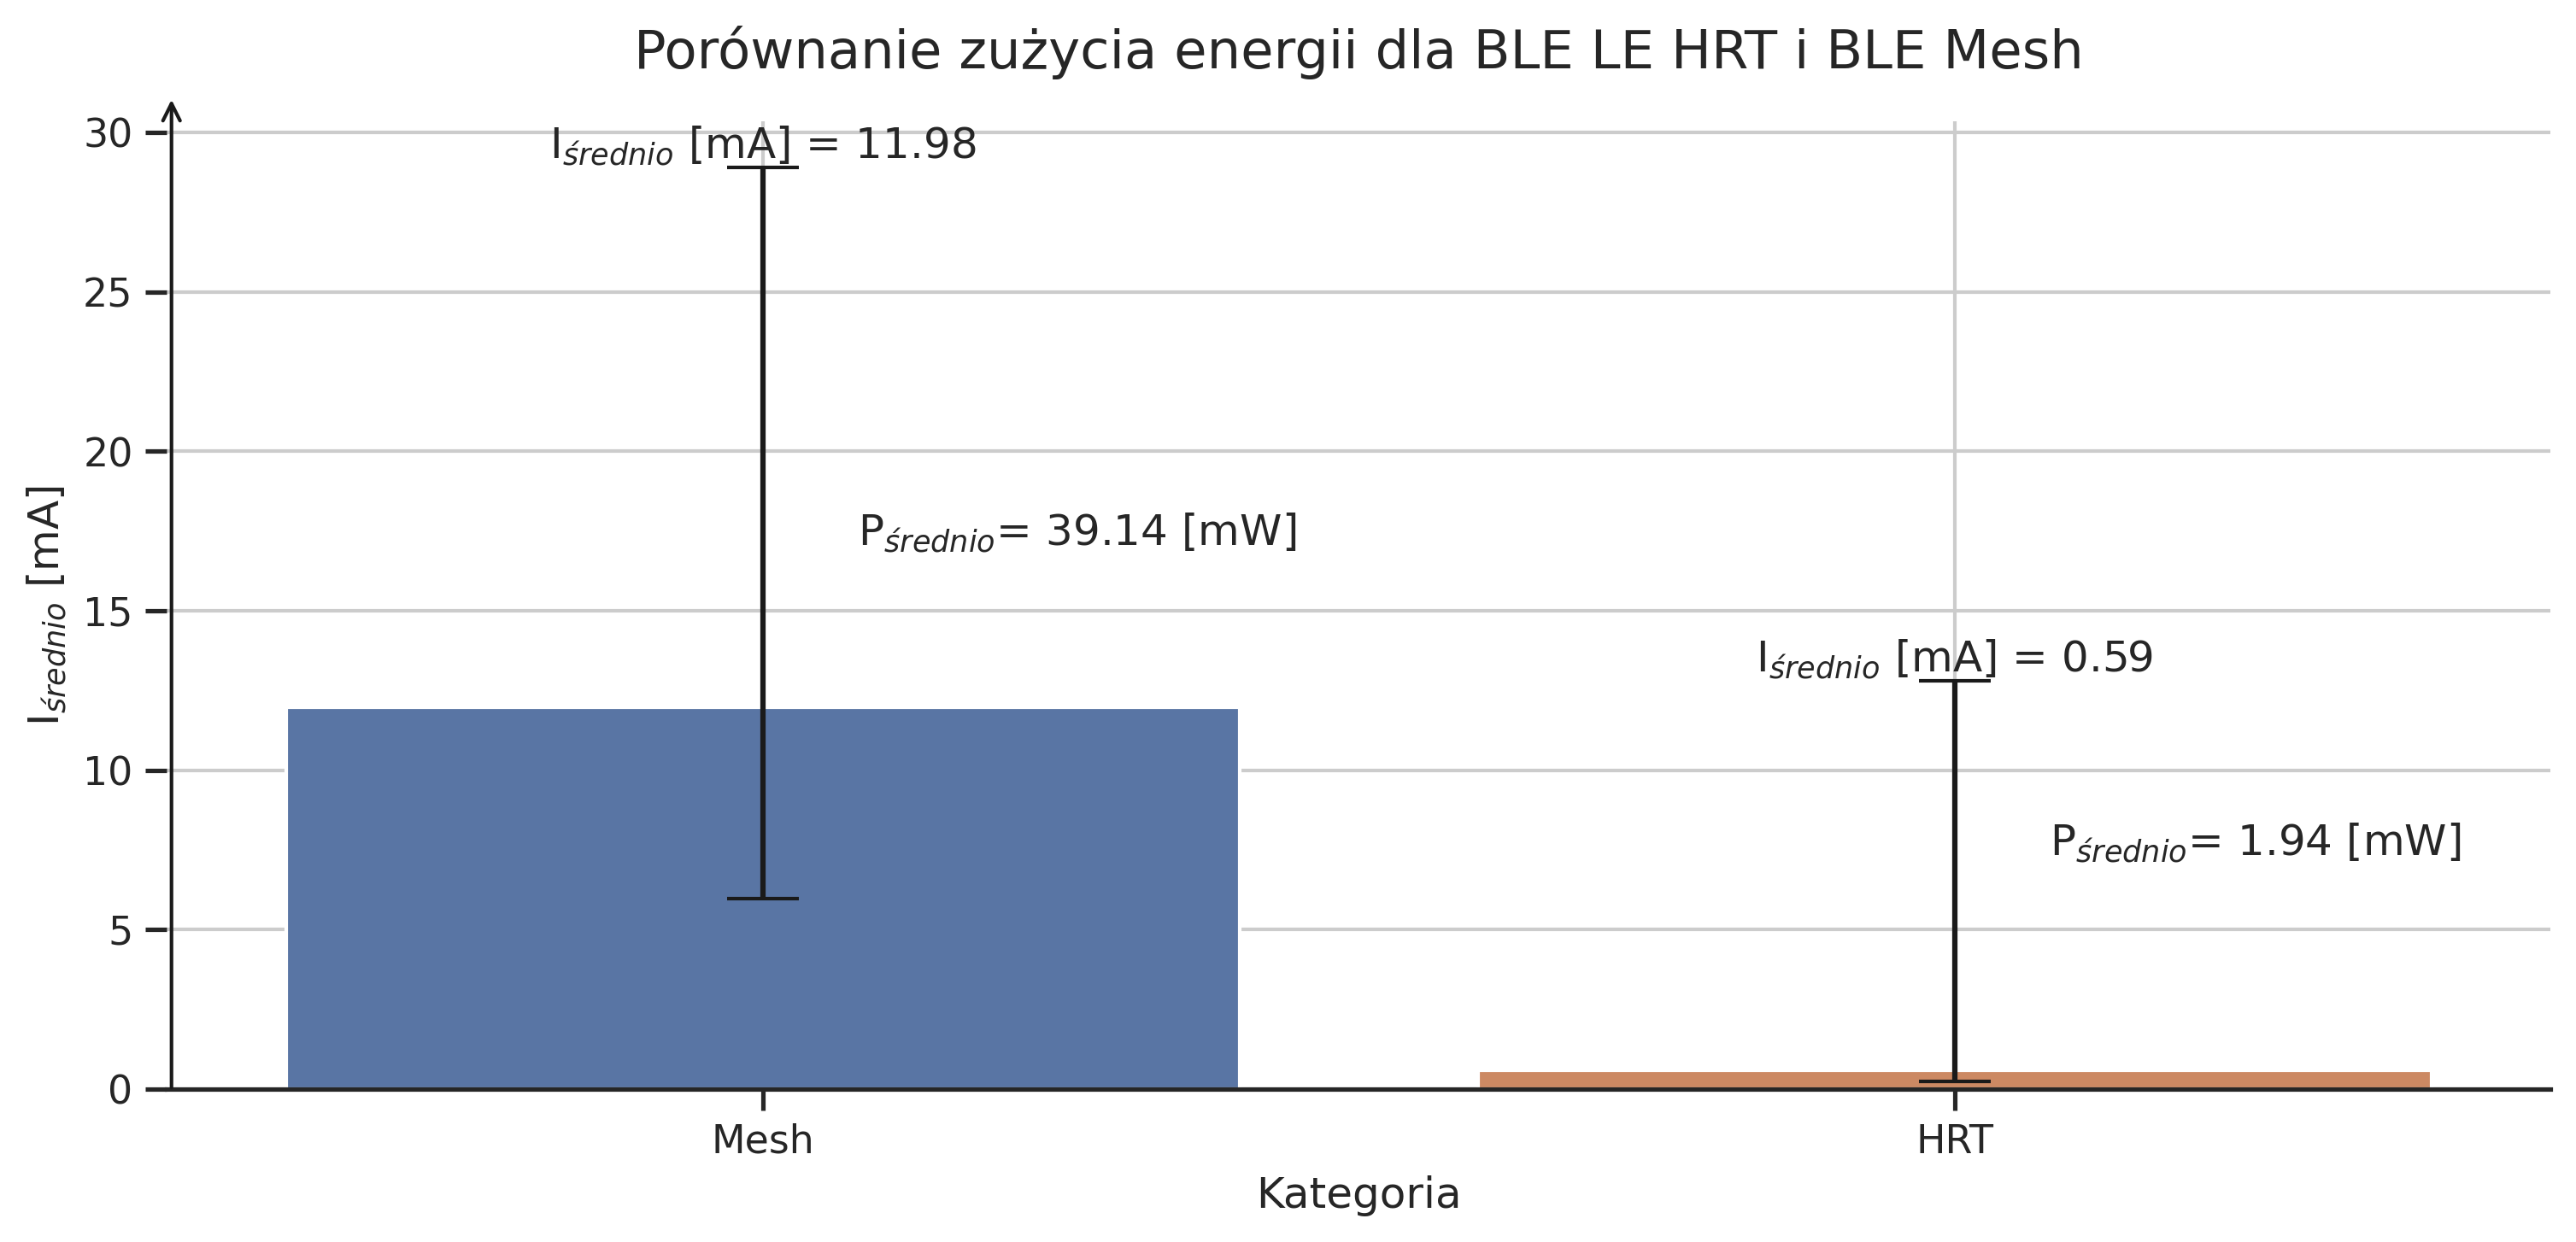
\includegraphics[width=0.99\linewidth]{power_ble_consumption_comparison_no_led.png} 
	\caption{Porównanie średniego zużycia energii pomiędzy BT Low Energy HRT i BLE Mesh}
	\label{rys:power_ble_consumption_comparison}
\end{figure}

W wykonanym doświadczeniu wykorzystano zwykły, prosty węzeł. Zapewniając niskie opóźnienia w~transmisji danych w~sieci, węzeł ten
spełnia inne zadania niż urządzenie oparte o~zwyczajne usługi BLE bądź węzeł LPN. Usługę BLE HRT zaprojektowano już na poziomie standardu
jako energooszczędne domyślnie. Urządzenie wykorzystujące takie usługi, będące najczęściej zasilanie bateryjnie, może działać
miesiące a nawet lata na pojedynczej baterii (np. typu pastylki CR2032). Dostrzeżona różnica jest więc oczekiwana, naturalna, wynikająca
z różnych przeznaczeń wykorzystywanych konfiguracji.
